\chapter*{CAPITULO III TITULO DEL CAPITULO}
\addcontentsline{toc}{chapter}{CAPITULO III TITULO DEL CAPITULO}
\setcounter{figura}{1}
\setcounter{tabla}{1}
%-------------------------------------------------------------------------
% Titulo de ejemplo 3.1
\section{3.1 Titulo de ejemplo 1}
Lorem ipsum dolor sit amet, consectetur adipiscing elit, sed do eiusmod tempor incididunt ut labore et dolore magna aliqua. Ut enim ad minim veniam, quis nostrud exercitation ullamco laboris nisi ut aliquip ex ea commodo consequat. Duis aute irure dolor in reprehenderit in voluptate velit esse cillum dolore eu fugiat nulla pariatur. Excepteur sint occaecat cupidatat non proident, sunt in culpa qui officia deserunt mollit anim id est laborum.

% Modificar "\newcommand{\descripcion}{....} para describir el contenido de la tabla.
% Modificar la fuente según corresponda. 
% Puede ajustar el tamaño de la figura modificando el parametro "scale", ej: 0.5 (1 corresponde al tamaño original)
\begin{figure}[H]
    \centering
    \newcommand{\descripcion}{Descripción de la figura.}
    \caption*{Figura \arabic{cap3}.\arabic{figura}: \descripcion}
    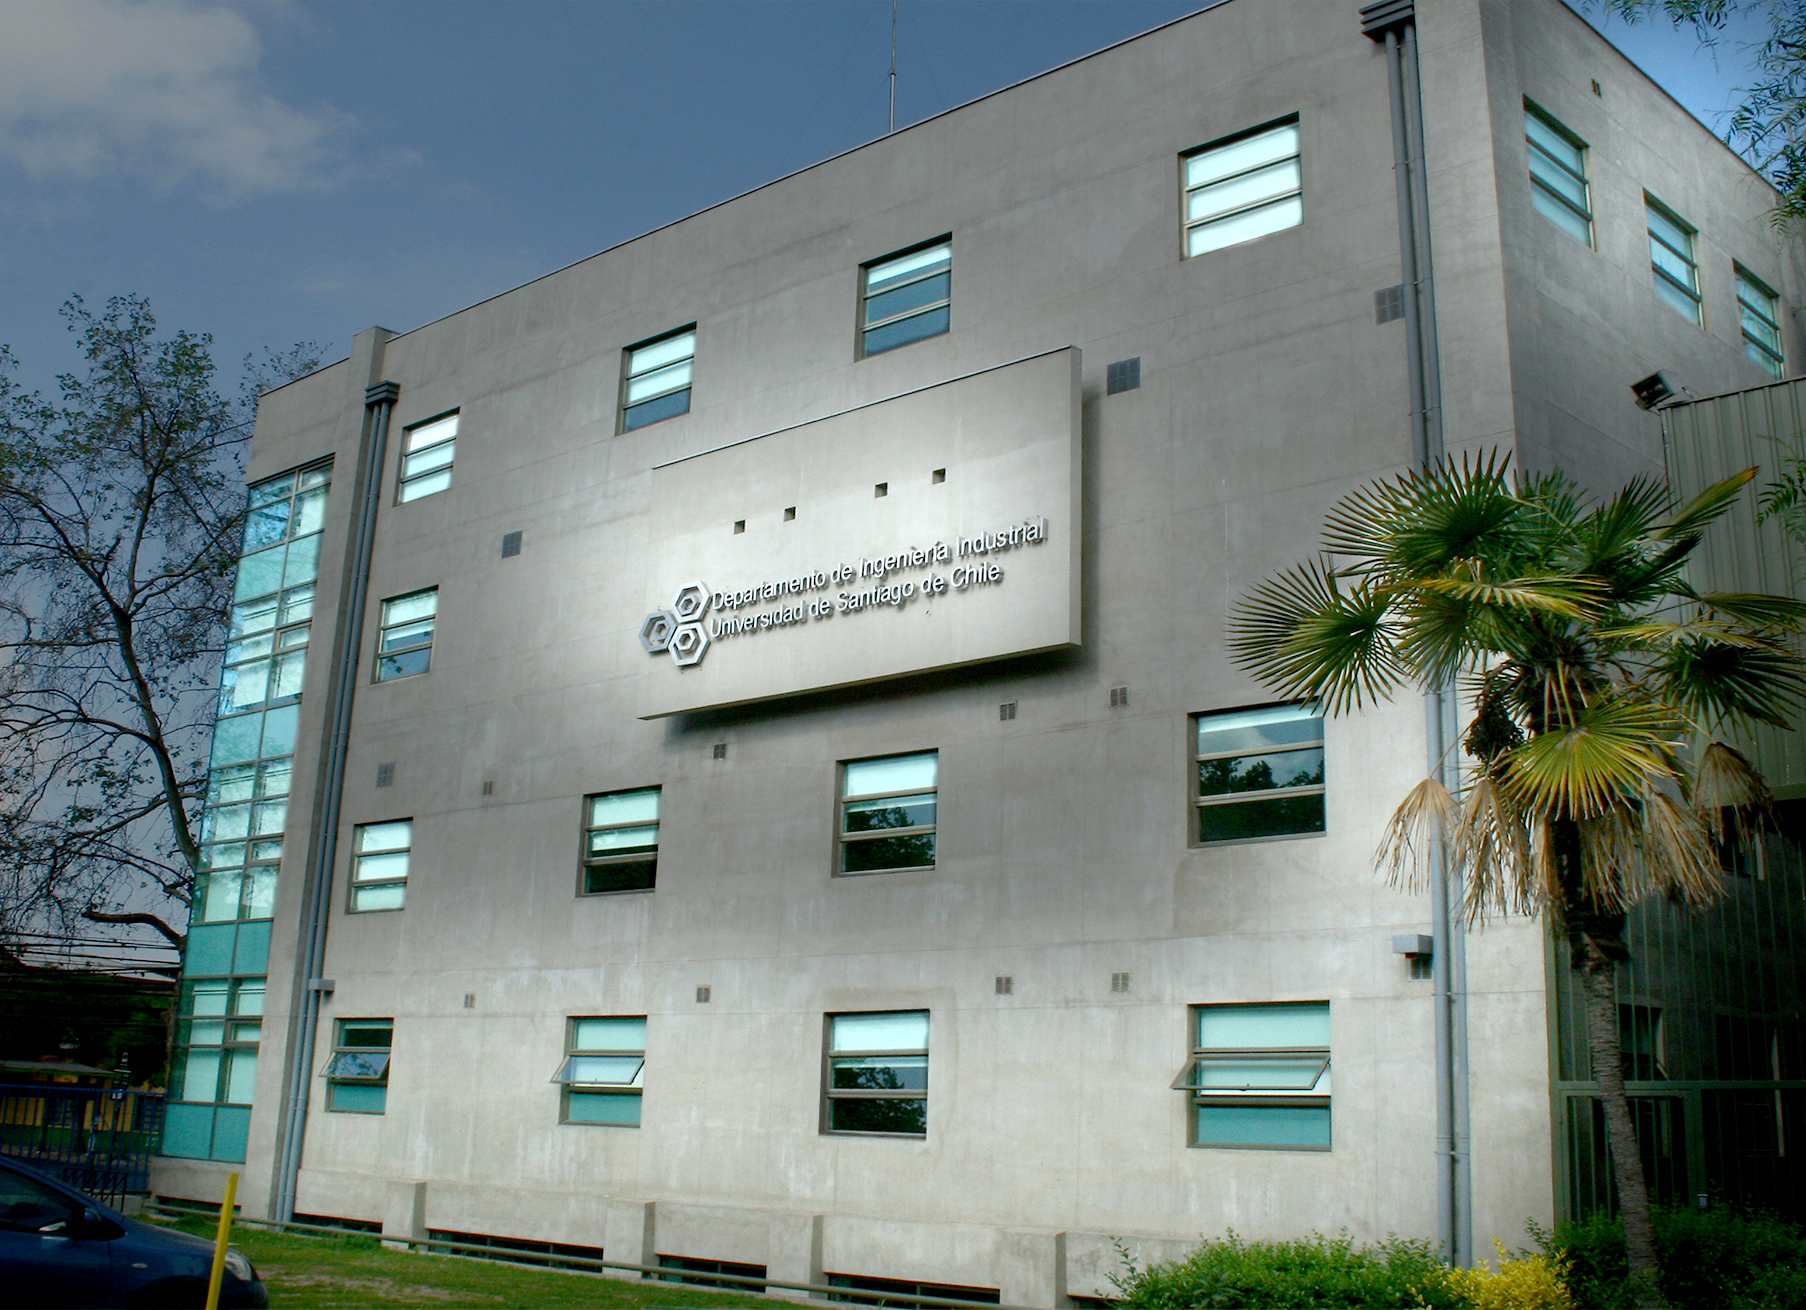
\includegraphics[scale=0.2]{figuras/dpto-industrias-usach.jpg}\\
    {\textit{\small Fuente: } \textit{\small Autores por apellido (año). Titulo del documento de donde se copio la figura.}}
    \label{fig:Dpto. Industrias 2}
    \addcontentsline{lof}{figure}{Figura \arabic{cap3}.\arabic{figura}: \descripcion}
    \addtocounter{figura}{1}
\end{figure}
% \label nos permite referenciar la tabla/figura en otra parte del documento.

%-------------------------------------------------------------------------
% Titulo de ejemplo 3.2
\section{3.2 Titulo de ejemplo 2}

% Modificar "\newcommand{\descripcion}{....} para describir el contenido de la tabla.
% Modificar la fuente según corresponda. 
% Puede ajustar el tamaño de la figura modificando el parametro "scale", ej: 0.5 (1 corresponde al tamaño original)
\begin{figure}[H]
    \centering
    \newcommand{\descripcion}{Descripción de la figura.}
    \caption*{Figura \arabic{cap3}.\arabic{figura}: \descripcion}
    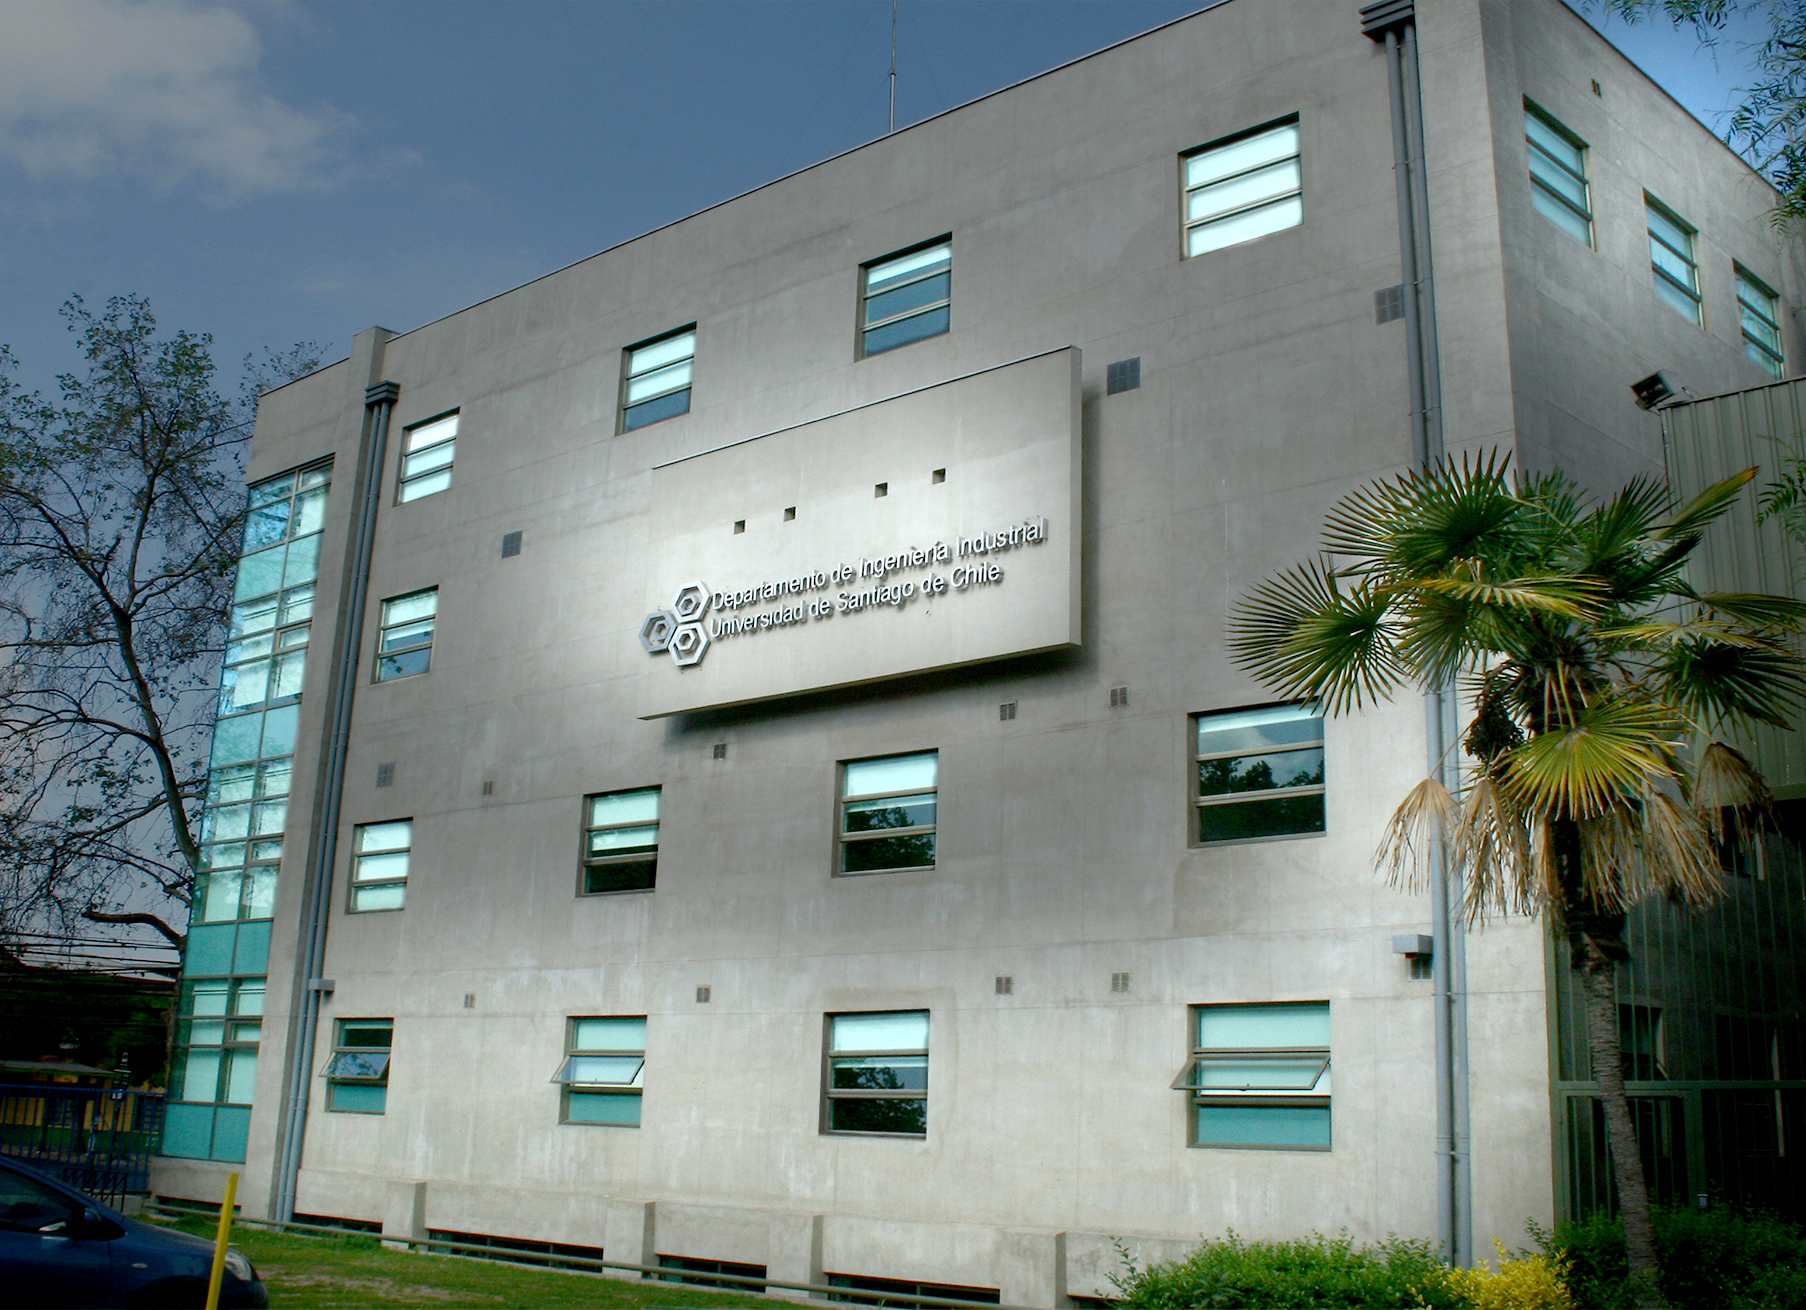
\includegraphics[scale=0.2]{figuras/dpto-industrias-usach.jpg}\\
    {\textit{\small Fuente: } \textit{\small Autores por apellido (año). Titulo del documento de donde se copio la figura.}}
    \label{fig:Dpto. Industrias 3}
    \addcontentsline{lof}{figure}{Figura \arabic{cap3}.\arabic{figura}: \descripcion}
    \addtocounter{figura}{1}
\end{figure}
% \label nos permite referenciar la tabla/figura en otra parte del documento.

Lorem ipsum dolor sit amet, consectetur adipiscing elit, sed do eiusmod tempor incididunt ut labore et dolore magna aliqua. Ut enim ad minim veniam, quis nostrud exercitation ullamco laboris nisi ut aliquip ex ea commodo consequat. Duis aute irure dolor in reprehenderit in voluptate velit esse cillum dolore eu fugiat nulla pariatur. Excepteur sint occaecat cupidatat non proident, sunt in culpa qui officia deserunt mollit anim id est laborum

%-------------------------------------------------------------------------
% Titulo de ejemplo 3.3
\section{3.3 Titulo de ejemplo 3}

Lorem ipsum dolor sit amet, consectetur adipiscing elit, sed do eiusmod tempor incididunt ut labore et dolore magna aliqua. Ut enim ad minim veniam, quis nostrud exercitation ullamco laboris nisi ut aliquip ex ea commodo consequat. Duis aute irure dolor in reprehenderit in voluptate velit esse cillum dolore eu fugiat nulla pariatur. Excepteur sint occaecat cupidatat non proident, sunt in culpa qui officia deserunt mollit anim id est laborum.

% Modificar "\newcommand{\descripcion}{....} para describir el contenido de la tabla.
% Modificar la fuente según corresponda. 
% Puede ajustar el tamaño de la figura modificando el parametro "scale", ej: 0.5 (1 corresponde al tamaño original)
\begin{figure}[H]
    \centering
    \newcommand{\descripcion}{Descripción de la figura.}
    \caption*{Figura \arabic{cap3}.\arabic{figura}: \descripcion}
    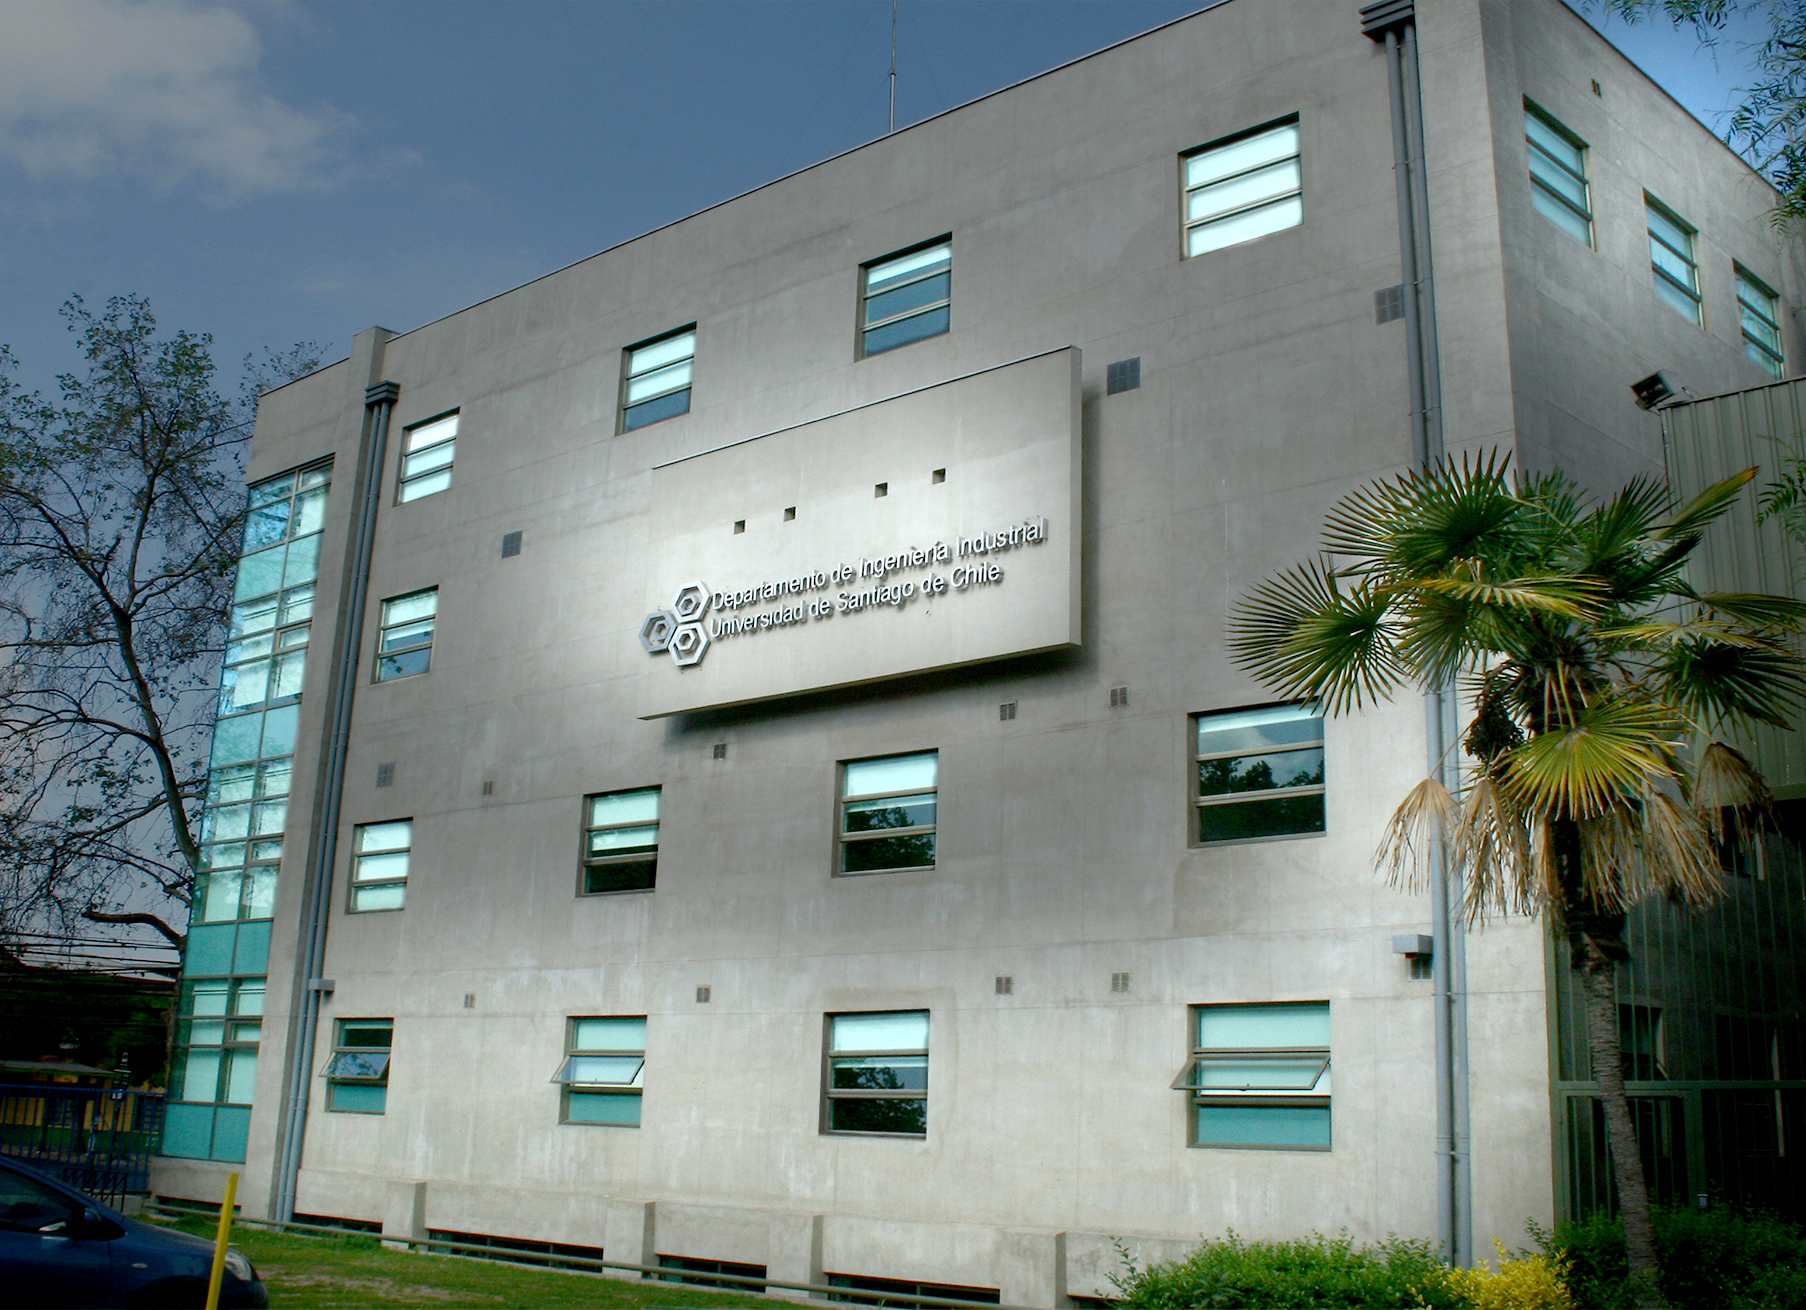
\includegraphics[scale=0.2]{figuras/dpto-industrias-usach.jpg}\\
    {\textit{\small Fuente: } \textit{\small Autores por apellido (año). Titulo del documento de donde se copio la figura.}}
    \label{fig:Dpto. Industrias 4}
    \addcontentsline{lof}{figure}{Figura \arabic{cap3}.\arabic{figura}: \descripcion}
    \addtocounter{figura}{1}
\end{figure}
% \label nos permite referenciar la tabla/figura en otra parte del documento.

En el caso de querer listar información de algún tipo, es posible hacerlo con 